\chapter{Methodology}

\label{chapter4}

In this chapter, we discuss about the techniques and methods used to devise an experiment involving a Pt-Cu bilayer system and subsequently investigate the effect of spin current via SHE.

\section{Experimental plan} \label{sec:plan}

In earlier studies, it has been shown that a pure spin current can be generated and manipulated via a heavy metal through SHE \cite{hirsch1999spin,sinova2004universal,zhang2000spin}. The detection of this spin current can only be done via conversion into charge current (which is measurable) using ISHE. This generally involves a ferromagnetic layer or a magneto-optical method \cite{kimura2007room,li2019spin,stamm2017magneto,valenzuela2007electrical}.

In our study, we intend to explore the detection of spin current in a NM/HM trilayer system without a magnetic layer, i.e. via electrical means such as using a simple voltmeter.

In many studies involving the electrical detection of spin current, pure spin current is generated using a ferromagnet at one end of the sample structure, which then gets converted to charge current via ISHE, and is subsequently, detectable using a voltmeter at the other end of the structure (which is usually a non-magnetic metal with high spin-orbit coupling).

Contrary to the above method, we do not generate pure spin current beforehand, but rather provide a pure charge current as supply to our sample, which is converted to spin current via SHE and is converted back to charge current via ISHE. Keeping this in mind, we design our sample accordingly.

\section{Preparation of sample}

We prepare a trilayer system, using copper (Cu) as the NM and platinum (Pt) as the HM. Here, we sandwich a layer of Cu between two layers of Pt. This is depicted in \cref{fig:layers}.

\begin{figure}
    \centering
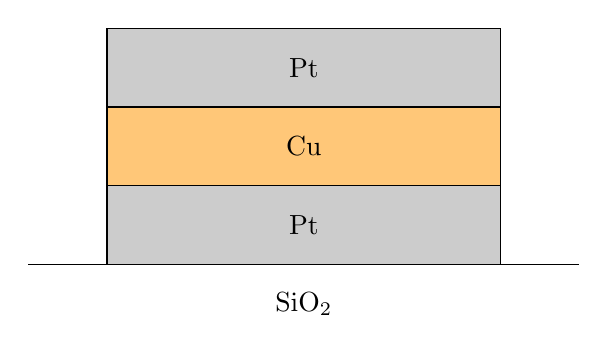
\begin{tikzpicture}
    \draw [fill={rgb:black,1;white,4}] (0,0) rectangle (5,3);
    \node at (2.5,2.5) {Pt};
    \draw [fill={rgb:orange,1;yellow,2;pink,5}] (0,0) rectangle (5,2);
    \node at (2.5,1.5) {Cu};
    \draw [fill={rgb:black,1;white,4}] (0,0) rectangle (5,1);
    \node at (2.5,0.5) {Pt};
    \draw (-1,0) -- (6,0);
    \node at (2.5,-0.5) {SiO$_2$};
\end{tikzpicture}
    \caption{Side view of the trilayer sample}
    \label{fig:layers}
\end{figure}

Now, as mentioned in \cref{sec:plan}, we intend to make the shape of our sample to facilitate the conversion to charge to spin current and vice versa.
As seen in \cref{sec:ishe} we see that converted spin current, flows perpendicular to the original charge current and similarly during the back conversion via ISHE.
For this, an obvious structural shape would be a path that has two paths, connected via a link being perpendicular to both the paths simultaneously.
Hence, a \textsc{H}-like structure comes to mind, which is implemented in our experimental setup.

\subsection{Fabrication of the sample}

Using the techniques of photolithography\footnotemark, magnetron sputtering\footnotemark[\value{footnote}] and focused ion beam\footnotemark[\value{footnote}], we fabricate our sample as depicted in \cref{fig:fabrication-sample}.

\begin{figure}
    \centering
    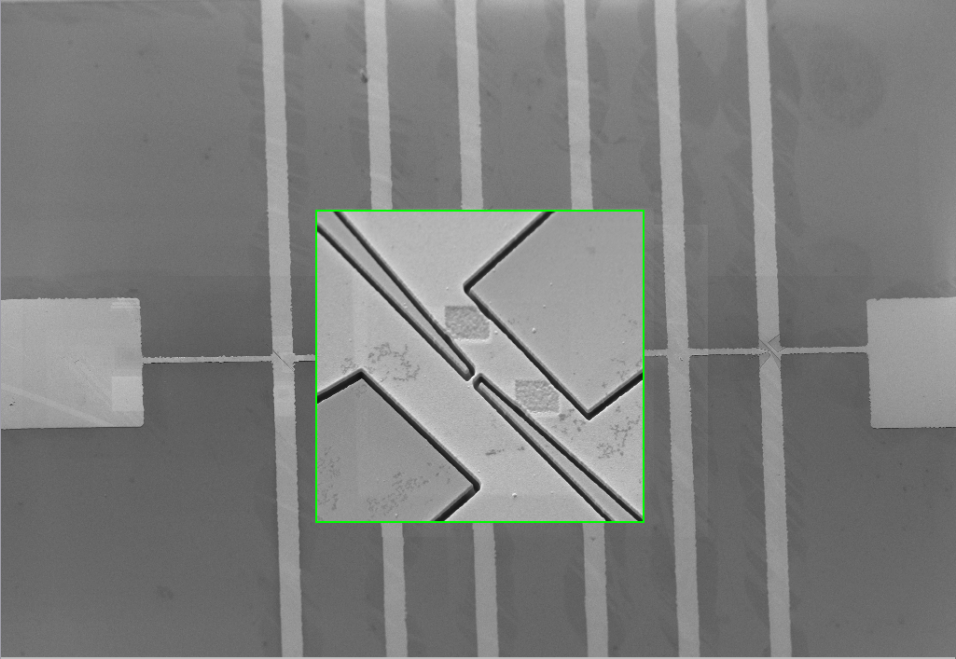
\includegraphics[scale=0.35]{newtrack.png}
    \caption{Patterned Cu/Pt sample used in the experimental setup.}
    \label{fig:fabrication-sample}
\end{figure}


\footnotetext{Details about these methods have been skipped for the sake of brevity.}

\subsection{Motivation behind choosing Pt and Cu}

One might wonder, why specifically did we choose Pt and Cu as our bilayer/trilayer sample?
We present the following reasons for choosing so:

\begin{itemize}
    \item In a lot of experiments involving SHE \cite{rojas2014spin,guo2008intrinsic,liu2011review,gladii2016spin}, Pt is used extensively due to its high spin Hall angle, which results from its high SOC.
        It also has good conductivity and is easy to grow onto thin films.

    \item Cu is used mainly because of its high spin diffusion length \cite{ramaswamy2017extrinsic}.
        This allows spin polarized electrons to maintain coherence for longer length scales.
\end{itemize}


\section{Detecting spin current}

In the case of OHE, the charge imbalance across the edges of the slab results in a potential difference (Hall voltage) \( V_H \) across the width of the sample.
This voltage can then simply be measured using a voltmeter.
But in the case of SHE, how does one go about measuring spin imbalance?
In such a case, there is no net charge transfer and hence conventional electrical measurements cannot be used directly.

One plausible way would be to use an instrument to measure the difference in localized magnetization across the width of the slab.
This can be achieved by using a superconducting quantum interference device microscope \cite{black1993magnetic} to measure local magnetic fields; the details into which we shall not go over for the sake of brevity.
A potential difficulty that arises in this approach would be to eliminate the contribution of magnetic field due to the longitudinal current density \( j_x \), it being greater in magnitude would mask the magnetization along the edges due to spin polarized electrons \cite{hirsch1999spin}.

We proceed to highlight a clever method to measure the spin current in a sample as proposed in \cite{hirsch1999spin}.

\begin{figure}[h!]
    \centering
    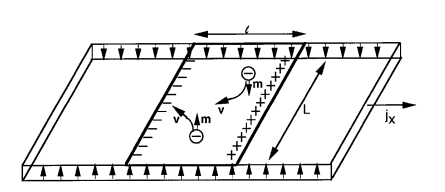
\includegraphics[scale=0.7]{hirsch.png}
    \caption{Schematic diagram depicting method to measurement of spin current.\\ \vspace{0.2cm} \textit{Image courtesy: JE Hirsch. ``Spin Hall effect" Phys. rev. letters (1999)}}
    \label{fig:hirsch-measure}
\end{figure}

The same scattering mechanisms (refer \cref{sec:mechanisms}) responsible for the conversion of charge current to spin current in the first place, will also be responsible for the conversion in the reverse direction i.e. ISHE.
This fact is exploited and we argue that by connecting a transverse strip across the slab would allow spin current to flow through it (as seen in \cref{fig:hirsch-measure}.

We take this strip made of a material (metal) with high SOC, only then can one observe ISHE to convert spin polarized electrons to a charge imbalance across width of strip.
Let charge current density \( j_x \) travel along the longitudinal direction.
The width of the slab is \( L \) and the width of the transverse strip is \( l \).
It is a necessary point to note that the width \( L \) cannot be more than the spin diffusion length \( \delta_s \) of the material of the slab.
\( \delta_s \) is the maximum length of a material, upto which spin coherence of spin polarized electrons is maintained.
Scattering mechanisms responsible for the phenomena, also lead to a loss of this spin coherence across a length scale given by \( \delta_s \), which is an intrinsic property of the material used.

As seen in the figure, charge current corresponding to \( j_x \) results in a spin imbalance across the edges of the slab due to SHE.
This results in spin current\footnote{Described in the preliminary sections (refer \cref{sec:she})}.

This spin current moves in a perpendicular direction compared to \( j_x \) but in the plane of the slab.
Via the same scattering mechanisms, the spin polarized electrons get preferentially scattered depending on the direction of their spins, resulting in a charge imbalance which is seen along the edges of the tranverse metal strip.
This charge imbalance gives rise to a potential difference across the strip, which can be measured by conventional electrical instruments such as a voltmeter.

\subsubsection{Mathematical formulation of spin voltage}

The magnetization of a sample with \( n_{\downarrow} \) as the number density of spin polarized (spin down) electrons is given by

\begin{equation}
    M = n_{\downarrow} \mu_B
\end{equation}

where \( \mu_B = \displaystyle \frac{e \hbar}{2 m_e}\) is the Bohr magneton.

Along with the longitudinal current density \( j_x \), we get an anomalous Hall voltage across the width of the sample as

\begin{equation} \label{eq:ano-hall-voltage}
    V_H = 4 R_s L j_x n_{\downarrow} \mu_B
\end{equation}

where \( R_s \) is the anomalous Hall coefficient and \( L \) is the transverse width of the slab.

\Cref{eq:ano-hall-voltage} can be extended for non-magnetic materials with high SOC, where the number density of spin \( \downarrow \) and spin \( \uparrow \) electrons is equal, giving rise to a ``spin Hall voltage'' \( V_{SH} \), whose sign depends on the direction of spin of the electrons.
This gives us the corresponding expression as,

\begin{equation} \label{eq:spin-voltage}
    V_{SH} = 2 \pi R_s L j_x n \mu_B
\end{equation}

where \( n \) is the total number density of conduction electrons and the rest of symbols have their usual meanings.

As described earlier, on connecting the edges of the slab via a tranverse strip of metal, the spin imbalance will cause a spin current to propagate in the metal strip.
The expression for spin current density is then written as

\begin{equation} \label{eq:j_eta}
    j_\eta = \frac{V_{SH}}{\rho L}
\end{equation}

where \( \eta \) is an index for each spin, \( \rho \) is the resistivity of the transverse strip.

As the spin current propagates through the strip, the spin polarized electrons get preferentially scattered via ISHE, leading to a charge imbalance across the strip.
This leads to a potential difference given by

\begin{equation} \label{eq:strip-voltage}
    V_{SH}^{\eta} = 4 \pi R_s l j_{\eta} n_{\eta} \mu_B
\end{equation}

where \( l \) is the width of the strip, \( j_{\eta} \) is the spin current density due to spin index \( \eta \), \( n_{eta} \) is the number density of electrons with spin index \( eta \).

Substitution of \cref{eq:j_eta} in \cref{eq:strip-voltage}, gives us the expression for voltage due to spin current, which can be measured using a simple voltmeter:

\begin{equation} \label{eq:spin-voltage2}
    V_{SC} = 8 \pi^2 R_s^2 l \frac{(n \mu_B)^2}{\rho} j_x
\end{equation}

Notice that in the above expression does not depend on the transverse width \( L \) anymore.
However, there is an implicit dependence on \( L \).
This is presented in the fact that if \( L \) is comparable to the spin diffusion length \( \delta_s \) of the slab, \( V_{SC} \) will decrease.

\subsubsection{Dependence of depth of slab on \( V_{SH} \) }

Let us analyze the dependence of width \( L \) of slab on \( V_{SH} \) from \cref{eq:spin-voltage}.
From the expression, the experimental parameters are \( L \) and longitudinal current density \( j_x \).
Let \( d \) be the depth of the slab and \( I_x \) be the charge current corresponding to \( j_x \).
Then, these quantities can be related as

\begin{equation*}
    j_x = \frac{I_x}{L d}
\end{equation*}

Substituting this value for \( j_x \) in \cref{eq:spin-voltage},

\begin{equation} \label{eq:spin-substitution}
    \begin{split}
        V_{SH} &= 2 \pi R_s L n \mu_B \left( \frac{I_x}{L d} \right)\\
               &= 2 \pi R_s n \mu_B \left( \frac{I_x}{d} \right)
    \end{split}
\end{equation}

Keeping the electrical current \( I_x \) constant throughout and taking \( k = 2 \pi R_s n \mu_B I_x \) as a constant, we rewrite \cref{eq:spin-substitution} as

\begin{equation} \label{eq:thin-slab}
    V_{SH} = \frac{k}{d} \quad \implies \boxed{V_{SH} \propto \frac{1}{d}}
\end{equation}

We see that the spin Hall voltage is inversely proportional to the depth of the sample used.
Therefore, to make a significant measurement, we require a thin slab.

\subsubsection{Extrapolation of \( V_{SC} \) via OHE}

\label{subsubsec:extrapolation}

In experiments involving the detection of spin current, an external magnetic field is not necessarily required but can be cleverly used.
Consider the case where an external magnetic field is supplied along the direction perpendicular to the plane of the slab in addition to \cref{fig:hirsch-measure}.

We know for a fact that due to OHE, a Hall voltage will be induced across the edges of the slab, which consequently results in a charge current along the transverse strip, giving an additional part to the spin voltage in \cref{eq:spin-voltage2}.
This total voltage is then given by \cite{hirsch1999spin} as

\begin{equation} \label{eq:vtb}
    V_t (B) = (R_0^2 B^2 + R_s^2 B_{eq}^2) \: \frac{l}{\rho} \: j_x
\end{equation}

where \( B_{eq} = 4 \pi n \mu_B / \sqrt{2} \), \( R_0 \) is the ordinary Hall coefficient and other symbols denote their usual meaning.

From an experimental perspective, it can be quite difficult to measure the spin current using this method, simply because the value of spin voltage is quite low for conventional voltmeters to be able to detect with significant precision.

To avoid this, an extrapolation technique involving OHE can be used, and is done as follows:
voltage measurements in the presence of an external magnetic field is done (given by \cref{eq:vtb}).
The data obtained can then be extrapolated to points where \( B = 0 \), which effectively reduces to the original scenario of measuring spin current without involving OHE.


\section{Measurement}

After the sample is prepared, we pass electrical (pure charge) current through one arm of the \textit{H}-structure and make voltage measurements across the opposite ends of the sample, as shown in \cref{fig:measurement}. This is technically called a non-local measurement.

\begin{figure}[!h]
\centering
    \begin{circuitikz}[american]
    \draw[thick] (0,0) rectangle (4,10);
    \draw[thick] (0,4.5) -- (-3,4.5);
    \draw[thick] (4,4.5) -- (7,4.5);
    \draw[thick] (0,6) -- (-3,6);
    \draw[thick] (4,6) -- (7,6);
    \draw[thick] (-3,4.5) -- (-3,6);
    \draw[thick] (7,6) -- (7,4.5);
    \draw (-3,5.25) -- (-4,5.25);
    \draw (-4,-1)
    to[isource, l=$I$] (-4,5.25);
    \draw (-4,-1) -- (2,-1);
    \draw (2,-1) -- (2,0);
    \draw (2,10) -- (2,11);
    \draw (2,11)
    to[V, l=$V$] (8,11);
    \draw (8,11) -- (8,5.25);
    \draw (8,5.25) -- (7,5.25);
    \begin{scope}[blue,xshift=-1.4cm,yshift=0.5cm,rotate=45]
        \draw (0,0) -- (4,0) -- (4,2) -- (0,2);
        \draw (10,0) -- (6,0) -- (6,2) -- (10,2);
        \draw (4.5,-3) -- (4.5,0.8) -- (5.5,0.8) -- (5.5,-3);
        \draw (4.5,5) -- (4.5,1.2) -- (5.5,1.2) -- (5.5,5);
    \end{scope}
    \end{circuitikz}
    \caption{Pure charge current is supplied across the left arm and the potential difference is measured across the right arm of the sample.}
    \label{fig:measurement}
\end{figure}

\subsection{Efficacy of the measurement}

\label{subsec:efficacy}

As seen in \cref{subsec:spin-angle}, the efficiency of conversion of spin current to charge current and vice versa is related to the spin Hall angle of the material.
However, this efficiency is very poor in practical laboratory environments.
Earlier studies in measuring spin current \cite{valenzuela2007electrical}, involved using a ferromagnetic layer to generate the spin polarized electrons, giving rise to spin current which is converted to charge current further down the experiment via ISHE.
In these studies, the conversion occurs only once, in contrast to our study where we do this to-and-fro conversion \textbf{twice}, meaning that the efficacy of measuring the spin current is much less as compared to traditional approaches \cite{valenzuela2007electrical}.

\subsection{Expected workflow}

As shown in \cref{fig:layer-workflow}, we provide an input current density \( J_c \), along one arm of the \Hst.

Referring back to \cref{fig:layers}, we see that the middle layer is Cu, sandwiched between two Pt layers at one end of the \Hst.

\begin{figure}
    \centering
    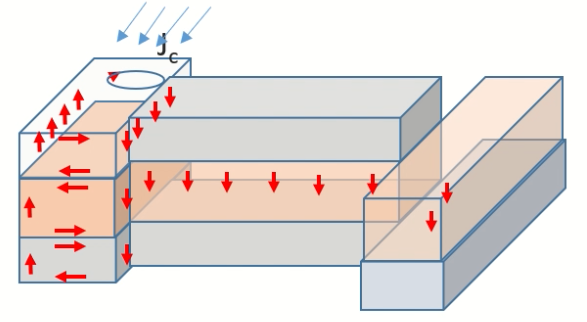
\includegraphics[scale=0.55]{current-layer.png}
    \caption{A schematic representation of the workflow of the experiment.}
    \label{fig:layer-workflow}
\end{figure}

We now proceed to describe, the step-by-step process of the expected phenomena:

\begin{enumerate}
    \item Input charge current density \( J_c \) moves through the first arm of the \Hst.
    \item Due to high SOC of Pt (the two outer layers), spin imbalance is observed along the edges of the Pt layers (via SHE), which then "seeps" into the Cu layer due to proximity effect. % TODO: Add footnote describing this phenomena.
    \item Cu being a good conductor and having high spin diffusion length (about 500 nm at room temperature \cite{Kimura_2005}), allows the spin current to propagate across the length of the arm-link layer, maintaining its spin.
    \item At the other end of the \Hst, charge imbalance is generated via ISHE, which then leads to a potential difference on the right arm (as seen in \cref{fig:layer-workflow}), which we measure non-locally using a voltmeter.
\end{enumerate}


\subsection{Final step}

After making the measurement of potential difference via voltmeter, the measurement readings are analyzed.\footnote{Done in the following chapter.}
